% -----------------------------*- LaTeX -*------------------------------
\documentclass[11pt]{report}
\usepackage{scribe_ds603}
\begin{document}

\scribe{Malay Kedia}		% required
\lecturenumber{17}			% required, must be a number
\lecturedate{Oct 29}		% required, omit year

\maketitle

% ----------------------------------------------------------------------

\section{Optimal Adversarial Loss}

We continue with the definition of Adversarial Risk defined in last class as:
\[
L_{N}(h)
    = \mathbb{E}_{(\vec{x}, y) \sim P^\ast}
      \!\left[
        \sup_{\vec{x}_{\text{adv}} \in N(\vec{x})}
        \ell\!\left((\vec{x}_{\text{adv}}, y), h\right)
      \right].
\]

\noindent
Consider the neighbourhood function:
\[
N(\cdot)
= 
\bigl\{\, \tilde{x} \;\text{s.t.}\; \| \tilde{x} - \cdot \|_2 \le \varepsilon \,\bigr\}.
\]

\noindent
For some classifier to be able to distinguish the 2 classes perfectly, the neighbourhoods of the points in opposite classes should not intersect. Conversely, if the neighbourhoods of 2 points in opposite classes intersect, there cannot exist a classifier which achieves an adverserial loss of 0.

\begin{figure}[ht]
    \centering
    \begin{minipage}{0.48\textwidth}
        \centering
        
\includegraphics[width=\linewidth]{images/img1.png}
    \end{minipage}\hfill
    \begin{minipage}{0.48\textwidth}
        \centering
        
\includegraphics[width=\linewidth]{images/img2.png}
    \end{minipage}
    \caption{Examples of 2 neighbourhood functions}
    \label{fig:side-by-side}
\end{figure}

\noindent
In the above example, there can exist an optimal classifier for \(N_1(\cdot)\) but not for \(N_2(\cdot)\). 

\noindent
\underline{Note:} Counting the number of intersections at the distribution level will tell us how many samples \emph{must} be misclassified.

\newpage
\subsection{Informal Theorem Statement}
For given class-wise distributions and a specified adversary, we have\\

\noindent
Lowest Robust Loss over a specific classifier family \(\;\ge\;\) Lowest Robust Loss over all possible classifiers

\vspace{5pt}
\noindent
where the lowest Robust Loss over all possible classifiers = a Simple function of an adversary-dependent distance between distributions. Moreover, there exists a classifier that achieves this optimal adversarial loss exactly.

\vspace{5pt}
\noindent
Note that this is significant because the lowest Robust Loss over a specific classifier family is very hard to calculate in general, but the lowest Robust Loss over all possible classifiers is a solution of convex program for continuous and discrete distributions of interest.

\noindent
\textbf{Can we relate the optimal adversarial risk to the optimal transport cost under the adversarial cost function? \cite{bhagoji2019lower} \cite{pydi2020adversarial}}

\subsection{Formal Theorem Statement}

\begin{theorem}
Consider the binary classification setting with \( Y \in \{0,1\} \),
where \( \vec{x} \) is drawn uniformly at random from \( P_0 \) and \( P_1 \).
The set of allowed hypotheses is \(\mathcal{H} := \{ h^A = \indic{A}(x \in A) : A \text{ is a closed set} \}\). Then, for the 0-1 loss function,
\[
\forall h^A \in \mathcal{H}, \quad L_N(h^A) \ge \frac{1}{2}\left[ 1 - D_{N_\varepsilon}(P_0, P_1) \right].
\]
Moreover, there exists some \( h^*_N \in \mathcal{H} \) that achieves the lower bound.
\end{theorem}

\subsection{Proof}

\begin{proof}
Let \( A \subseteq \mathcal{X} \) be a closed set where the classifier declares \( 1 \) on \( A \) and \( 0 \) elsewhere. Then,

\begin{align*}
\inf_{h^A \in \mathcal{H}} L_N(h^A)
&= \inf_{A \text{: closed}}
    \frac{1}{2}\!\left( P_0(A^\varepsilon) + P_1\big((A^c)^\varepsilon\big) \right) \nonumber\\[0.6em]
&= \frac{1}{2}\!\left( 1 - \sup_{A \text{: closed}}
    \big[ P_1\big(\big((A^c)^\varepsilon)\big)^c\big - P_0(A^\varepsilon) \big] \right) \nonumber \quad \quad  \text{by Law of Total Probability}\\[0.6em]
\end{align*}

\noindent
where, \( A^\varepsilon \) denotes the \emph{expansion} of a set \( A \), defined as
\[
A^\varepsilon = \{ \vec{x} \in \mathcal{X} : d(\vec{x}, \vec{x}') \le \varepsilon \text{ for some } \vec{x}' \in A \}.
\]
We also define
\[
A^{-\varepsilon} = \left( (A^c)^\varepsilon \right)^c.
\]

\newpage
The following properties hold for Set Expansions and Complements:

\begin{center}
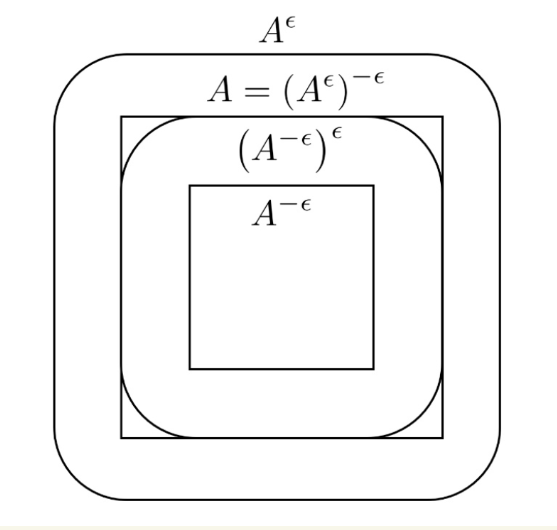
\includegraphics[width=0.4\textwidth]{images/img3.png}
\end{center}


\begin{itemize}
    \item \( ((A^{-\varepsilon})^\varepsilon = (((A^c)^\varepsilon)^c)^\varepsilon \subseteq A \)
    \item \( A \subseteq (A^\varepsilon)^{-\varepsilon} \) and  \((A^\varepsilon)^{-\varepsilon} \subseteq A \;\;\). So,  \((A^\varepsilon)^{-\varepsilon} = A \)
    
\end{itemize}

\begin{theorem}[Strassen's Theorem]
Let $\mathcal{X}$ be a Polish space, and let $P, Q$ be probability measures on $\mathcal{X}$ with $\varepsilon > 0$. Then
\begin{align*}
D_{N_{\frac{\varepsilon}{2}}}(Q, P)
&= \inf_{\pi \in \Pi(Q, P)} \mathbb{E}_{(\vec{x}, \vec{x}') \sim \pi}\!\left[\, \mathds{1}( d(\vec{x}, \vec{x}') > \varepsilon ) \,\right]\\
&= \inf_{\pi \in \Pi(Q, P)} \pi \!\left[\, \{ (\vec{x},\vec{x}') \;|\;  d(\vec{x}, \vec{x}') > \varepsilon \} \,\right]\\[0.5em]
&\ge \sup_{A \text{: closed}} \big[ Q(A) - P(A^\varepsilon) \big],
\end{align*}
and some closed set \(A\) achieves the supremum.
\end{theorem}

\smallskip
\noindent
\underline{Note:} This is a special case of \emph{Kantorovich duality}, which states that for lower semicontinuous cost functions \(c(x, y)\), and for functions \(\alpha(\cdot)\) and \(\beta(\cdot)\) satisfying \(\alpha(\vec{x}') - \beta(\vec{x}) \le c(\vec{x}, \vec{x}') \;\; \forall \vec{x}, \vec{x}'\),
\[
\inf_{\pi \in \Pi(Q, P)} \mathbb{E}_\pi[c(x, x')]
= \sup_{\alpha, \beta} \big( \mathbb{E}_P[\alpha(\vec{x}')] - \mathbb{E}_Q[\beta(\vec{x})] \big).
\]

% \subsection*{Key Question}
% Why is the equivalence between \emph{optimal robust loss} and \emph{optimal transport} with a specific loss function important?

\medskip
\noindent
Coming back to the proof of the equivalence, it suffices to show that
\begin{align*}
\sup_{A \text{: closed}} \big[ P_1(A^{-\varepsilon}) - P_0(A^\varepsilon) \big]
= \sup_{A \text{: closed}} \big[ P_1(A) - P_0(A^{2\varepsilon}) \big].
\end{align*}

\begin{lemma}
If \(A\) is closed, then both \(A^{\varepsilon}\) and \(A^{-\varepsilon}\) are closed.
\label{lemma1}
\end{lemma}

\begin{lemma}
Let \(A\) be closed. Then
\((A^{-\varepsilon})^{\varepsilon} \subseteq A\) and \(A \subseteq (A^{\varepsilon})^{-\varepsilon}\).
\label{lemma2}
\end{lemma}

\subsubsection{Proof of Inequality Direction 1 (\( \text{RHS} \ge \text{LHS} \))}

\begin{align*}
\sup_{A \text{: closed}} \big[ P_1(A) - P_0(A^{2\varepsilon}) \big]
&\ge \sup_{A \text{: closed}} \big[ P_1(A^{-\varepsilon}) - P_0((A^{-\varepsilon})^{2\varepsilon}) \big] \\
&\ge \sup_{A \text{ closed}} \big[ P_1(A^{-\varepsilon}) - P_0(A^{\varepsilon}) \big],
\end{align*}
where the first step is a variable substitution which follows from \ref{lemma1} and last step follows from \ref{lemma2}:
\[
(A^{-\varepsilon})^{2\varepsilon} = \big( (A^{-\varepsilon})^{\varepsilon} \big)^{\varepsilon}
\subseteq A^{\varepsilon}.
\]
Thus, \(P_0((A^{-\varepsilon})^{2\varepsilon}) \le P_0(A^{\varepsilon})\).


\subsubsection{Proof of Inequality Direction 2 (\( \text{LHS} \ge \text{RHS} \))}

\begin{align*}
\sup_{A \text{: closed}} \big[ P_1(A^{-\varepsilon}) - P_0(A^\varepsilon) \big]
&\ge \sup_{A \text{: closed}} \big[P_1((A^{\varepsilon})^{-\varepsilon}) - P_0((A^{\varepsilon})^{\varepsilon})\big] \\
&\ge \sup_{A \text{: closed}} \big[ P_1(A) - P_0(A^{2\varepsilon})\big]
\end{align*}

\noindent
where first step is a variable substitution, and second step follows from \ref{lemma2}.

\smallskip
\noindent
Now, by Strassen’s theorem and the definition of \( D_N^\varepsilon(P_0, P_1) \),
\begin{align*}
\inf_{h^A \in \mathcal{H}} L_N(h^A)
&= \frac{1}{2}\!\left( 1 - \sup_{A \text{: closed}} \big[ P_1(A^{-\varepsilon}) - P_0(A^{\varepsilon}) \big] \right) \\[0.6em]
&= \frac{1}{2}\!\left( 1 - \sup_{A \text{: closed}} \big[ P_1(A) - P_0(A^{2\varepsilon}) \big] \right) \\[0.6em]
&= \frac{1}{2}\!\left( 1 - D_{N_\varepsilon}(P_0, P_1) \right).
\end{align*}

\end{proof}

\begin{corollary}[Link to the Wasserstein Distance]


Under the same conditions as the preceding theorem, we have
\[
\inf_{h^A \in \mathcal{H}} L_N(h^A)
\ge
\frac{1}{2} \left[ 1 - \left( \frac{W_r(P_0, P_1)}{2\varepsilon} \right)^{\!r} \right],
\]
where \(W_r(P_0, P_1)\) denotes the \(r\)-th Wasserstein distance.
\medskip
\end{corollary}

\begin{proof}
Let \(r \ge 1\). For any \(\pi \in \Pi(P_0, P_1)\),
\begin{align*}
\mathbb{E}_\pi\!\left[\mathds{1}\{ d(\vec{x}, \vec{x}') > 2\varepsilon \}\right]
&= \mathbb{P}_\pi\!\big[\, d(\vec{x}, \vec{x}') > 2\varepsilon \,\big]\\
&= \mathbb{P}_\pi\!\big[\, d^r(\vec{x}, \vec{x}') > (2\varepsilon)^r \,\big]\\
&\le
\frac{\mathbb{E}_\pi[\, d(\tilde{x}, \tilde{y})^r \,]}{(2\varepsilon)^r}.
\end{align*}

\noindent
Therefore,
\[
\inf_{\pi \in \Pi} \mathbb{E}_\pi\!\left[\mathds{1}\{ d(\tilde{x}, \tilde{y}) > 2\varepsilon \}\right]
\le
\frac{\inf_{\pi \in \Pi} \mathbb{E}_\pi[\, d^r(\vec{x}, \vec{x}') \,]}{(2\varepsilon)^r}
= \frac{W_r(P_0, P_1)^r}{(2\varepsilon)^r}.
\]
\end{proof}
\subsection{Empirical Results}

We now empirically compare the optimal minimum adversarial loss (derived theoretically)
with the robust loss achieved by trained classifiers under adversarial attacks.

\subsubsection{Experimental setup}

\begin{itemize}
    \item Train a robust classifier using Projected Gradient Descent (PGD) to maximize a proxy loss:
    \begin{equation*}
        h_{\text{robust}}
        = \min_h \;
        \mathbb{E}\!\left[
            \max_{\|\delta\| \le \varepsilon} 
            L_{\text{proxy}}\big((x + \delta, y), h\big)
        \right].
    \end{equation*}

    \item Compute the loss on the training data using PGD attacks for different perturbation radii~$\varepsilon$.
    
    \item Compute the optimal minimum loss using minimum matching on a bipartite graph,
    which corresponds to the optimal transport solution between class distributions.
\end{itemize}

\subsection*{Results}

\begin{figure}[h!]
    \centering
    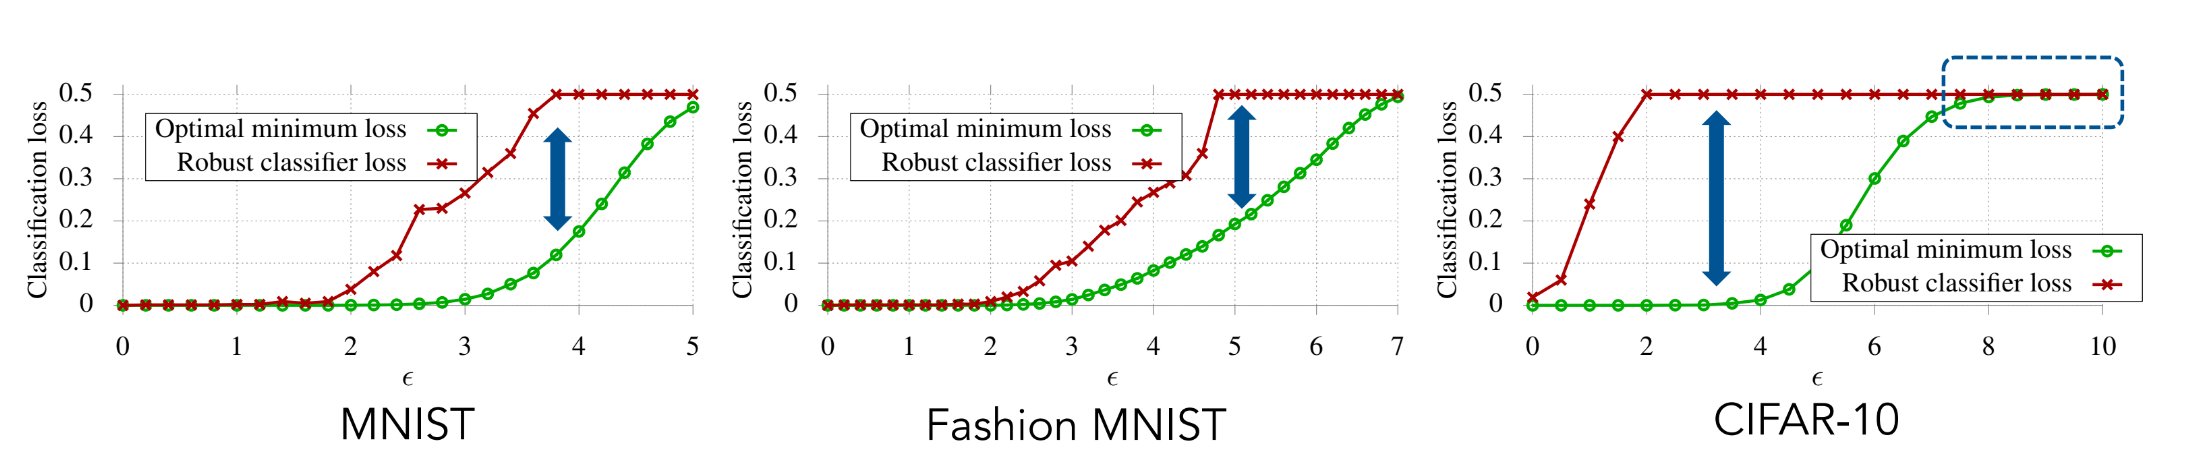
\includegraphics[width=1.1\textwidth]{images/img4.png}
\end{figure}

\subsubsection{Observations and Takeaways}

\begin{itemize}
    \item There is a large gap between the optimal and learned (PGD-trained) robust losses,
    which increases with~$\varepsilon$.
    \item For large~$\varepsilon$, correct classification becomes impossible,
    as both the learned and optimal losses approach~$0.5$ (random guessing performance).
\end{itemize}

\bibliographystyle{plain}
\bibliography{refs}

\end{document}